\documentclass{article}
\usepackage[UTF8]{ctex} % 用于中文排版
\usepackage{geometry}
\usepackage{indentfirst}
\usepackage{enumitem}

\usepackage{titling}    % 用于自定义标题页
\usepackage{graphicx}
\usepackage{subfigure}
\usepackage{float}

\usepackage{xcolor}
\usepackage{listings}

\usepackage{setspace}

% 页面几何设置
\geometry{a4paper, left=25mm, right=25mm, top=25mm, bottom=25mm}
% 取消首行缩进
\setlength{\parindent}{0pt}
% 行间距设置
\setstretch{1.5}
% 自定义字体大小
\newcommand{\fourhao}{\fontsize{14pt}{\baselineskip}\selectfont} % 四号字体
\newcommand{\xiaosihao}{\fontsize{12pt}{\baselineskip}\selectfont} % 小四号字体
\newcommand{\song}{\CJKfamily{song}}
% 设置代码块格式
\lstset{
    basicstyle = \footnotesize\ttfamily,                 % 设置行距,字体
    numbers = left,                                      % 在左侧显示行号
    numberstyle = \tiny \color{gray},                    % 设定行号格式
    keywordstyle = \bfseries \color[RGB]{40,40,255},     % 设定关键字颜色
    numberstyle = \footnotesize \color{darkgray},           
    commentstyle = \color[RGB]{0,96,96},                 % 设置代码注释的格式
    stringstyle = \color[RGB]{128,0,0},                  % 设置字符串格式
    frame = single,                                      % 不显示背景边框
    backgroundcolor = \color[RGB]{245,245,244},          % 设定背景颜色
    language=Verilog                                     % 设置语言
}
\raggedbottom   % 段落间留白, 避免排版时自动拉伸导致的行间距变化。
\begin{document}

% 封面页面
\begin{titlepage}
    \centering
    \vspace*{2cm}

    \Huge
    \textbf{课程名称:EDA 技术综合设计}

    \vspace{2cm}

    \LARGE
    设计报告名称:设计四\ 任意小数和整数分频器设计

    \vspace{4cm}

    \centering
    \Large
    \begin{tabular}{rl}
        班级: & 通信214    \\
        姓名: & \ 王峤宇   \\
        学号: & \ 214022
    \end{tabular}

    \vfill

    \vspace{1cm}
\end{titlepage}

\newpage
% 第一部分
\section*{\fourhao 一、设计内容及原理}
\xiaosihao
\setstretch{1.5}
% 设计项目内容及设计原理,如真值表、状态表及状态转换图、文字说明等。
\subsection*{设计内容}
寄存器是用来存储二进制信息的电路。有存储功能和移位功能, 是最基本的时序逻辑电路设计元件。
\subsection*{基础任务}
\textbf{设计任务}:数码管显示时,肉眼能分辨的频率在30多赫兹左右最好,对100MHz的时钟分频,分频到肉眼可见的频率范围。
输出频率时钟由发光二极管显示,同时由数码管显示分频系数。需要给出计算过程。\\

\textbf{时钟分频}: 分频采用DDS中的频率控制字实现任意分频效果的思路完成, DDS中的通过频率控制字控制相位累加器的累加步长, 
实现任意频率相位信号输出。具体计算如下:\\
假设FPGA的基准频率为100MHz:
\begin{equation}
    f_c = 1*10^8 (Hz)
\end{equation}
假定计数器为32位计数器, 总的频率控制字上限为计数器计数值的一半, 也就是最小为2分频, 最大输出为输入时钟的一半, K为频率控制字, 计算过程如下:
\begin{equation}
    N = 2^{32}
\end{equation}
\begin{equation}
    f_o = \frac{f_c*K}{N} = 0.023283 * K
\end{equation}
可以实现频率分辨率为0.024的任意频率输出。最小频率为0.023283Hz输出, 最大频率为输入时钟的一半, 即50MHz。
通过可以得到, 为了得到大概30Hz的输出, K值取为:
\begin{equation}
    K = \frac{f_o}{0.023283} = 1288
\end{equation}
此时的理论输出频率为:29.9886Hz, 实现输入信号的3,334,601.9分频。
\begin{equation}
    f_o = \frac{f_c*K}{N} = 0.023283 * 1288 = 29.9886Hz
\end{equation}
\subsection*{提高内容}
\textbf{设计任务}:设计一个偶分频的通用分频器(通用值 N),输出频率时钟由发光二极管显示,同时由数码管显示分频系数。
N值由外部拨码开关输入。\\

\textbf{偶数分频器设计}:数倍分频是最简单的一种分频模式,可以直接通过计数器计数实现。计数器由输入时钟的上升沿或下降沿驱动, 
从0开始, 向上计数当计数值达到N - 1时清零, 实现一个周期, 其中小于N/2的部分和小于N的部分对称, 通过组合逻辑判断计数值就可以
实现偶数倍的分频。
\subsection*{拓展任务}
\textbf{任务要求}:设计一个奇分频的通用分频器(通用值 N),输出频率时钟由发光二极管显示,同时由数码管显示分频系数。
N 值由外部拨码开关输入。\\

\textbf{奇数分频器设计}:奇数分频器通常由两个计数器实现, 将产生的两个时钟进行组合逻辑运算得到相应的50\%占空比的分频信号输出。\\
\subsubsection*{两个计数器输出进行或运算}
一个计数器计数信号的上升沿, 对信号进行N分频, 另一个计数器采样信号的下降沿, 同样对信号进行N分频, 产生不为50\%的波形, 以3分频为例, 计数器包含计数值0, 1, 2三个值, 通过组合逻辑电路使其在
0, 1状态时输出clk为高电平, 值为2时输出clk为低电平, 这样就会导致高电平的时间大于低电平时间一个周期, 此时通过另一个下降沿采样计数器同理产生相应的时钟, 由于对下降沿采样, 在输入时钟严格保证50\%占空比时, 第二个时钟相比第一个是时钟延迟了半个时钟周期, 
对连个时钟进行或操作得到的结果, 使得高电平时间增加半个周期, 低电平时间减少半个周期, 这样就实现了奇数分频中奇数周期的平分, 使得高电平为1.5个周期, 低电平也为1.5个周期的50\%占空比分频。 
\subsubsection*{设计完整系统}
针对基础任务、提高任务和拓展任务的三者进行结合设计, 设计得到的该系统中, 支持8位二进制0~255的分频系数设置, 当选择0或1时, 为不分频, 输出结果为30Hz的时钟, 数码管显示对应的分频系数, 
直接进行通过拨码开关设置指定的分频系数, 系统对30Hz的时钟进行分频, 方便观察, 实现奇数分频和偶数分频。\\
\begin{figure}
    \centering
    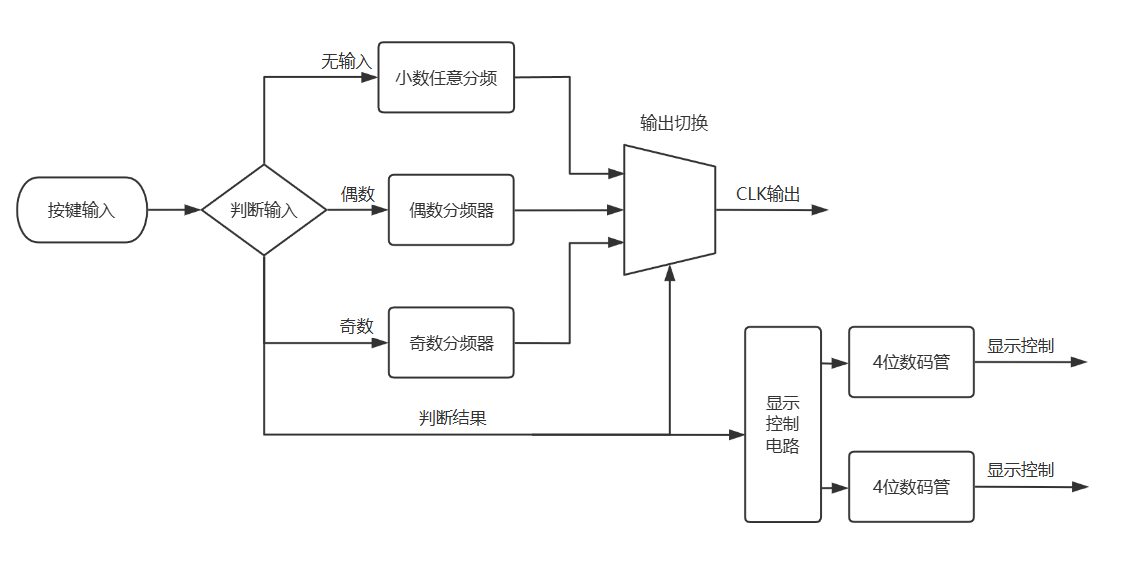
\includegraphics[width=0.7\textwidth]{image/2024-06-28-15-55-33.png}
    \caption{完整系统模块框图}
    \label{image_principle_1}
\end{figure}
将小数任意分频、奇数分频、偶数分频模块合并, 实现不同输入不同输出的分频系统, 其模块框图如图\ref{image_principle_1}所示。
% 第二部分
\section*{\fourhao 二、设计过程}
\xiaosihao
\setstretch{1.5}
% 从工程建立开始,一直到硬件调试。
% 按照基础任务、提高任务和拓展任务分别给出相应的源文件、仿真文件、约束文件
\subsection*{基础任务}
通过DDS中相位累加器实现的任意分频器源文件如下:
\begin{lstlisting}[language=Verilog, caption={任意分频器代码}]
module clk_div_32bit(
    input clk,
    input rstn,
    input [31:0] step_freq,
    output clk_out
    );
    /* 相位累加器 */
    reg [31:0] cnt = 32'b0;
    always@(posedge clk or negedge rstn) begin
        if(!rstn)  
            cnt <= 32'b0;
        else  
            cnt <= cnt + step_freq;
    end
    /* 相位波形输出, 由于实现的是分频, 输出为50占空比的方波 */
    reg cnt_equal;
    always @(posedge clk or negedge rstn) begin
        if (!rstn) begin
            cnt_equal <= 1'b0;
        end else if(cnt < 32'h8000_0000) begin
            cnt_equal <= 1'b0;
        end else begin
            cnt_equal <= 1'b1;  
        end
    end
    assign clk_out = cnt_equal;
endmodule
\end{lstlisting}
实现任意分频, 同时显示分频系数的top文件代码如下, 分频系数固定, 直接采用数码管输出。
\begin{lstlisting}[language=Verilog, caption={基础任务top源文件}]
module clk_div_top(
    input clk,                  /* 100MHz */
    input rst,                  /* 低电平异步复位 */
    input [7:0] div_coe,        /* 输入的四位整数加四位小数的二进制实数 */
    output [7:0] sseg1, sseg2,  /* 八段数码管 */
    output [3:0] an1, an2,      /* 片选信号 */
    output led_out              /* 闪烁的LED灯 */
    );
    /* 分频, */
    clk_div_32bit  clk_div_32bit_inst (
        .clk(clk),
        .rstn(!rst),
        .step_freq(32'd1288),
        .clk_out(led_out)
    );
    /* 第一个四位数码管 */
    scan_led_hex_disp_4  scan_led_hex_disp_4_inst_0 (
        .clk(clk), .rst(rst),
        .hex0(4'd3), .hex1(4'd3), .hex2(4'd3), .hex3(4'd4), .dp(4'b0000),
        .an(an1), .sseg(sseg1)
    );

    /* 第二个四位数码管 */
    scan_led_hex_disp_4  scan_led_hex_disp_4_inst_1 (
        .clk(clk), .rst(rst),
        .hex0(4'd6), .hex1(4'd0), .hex2(4'd1), .hex3(4'd9), .dp(4'b0010),
        .an(an2), .sseg(sseg2)
    );
endmodule
\end{lstlisting}
Top系统仿真文件如下:
\begin{lstlisting}[language=Verilog, caption={top仿真文件}]
module clk_div_top_tb_1;
    reg  clk;
    reg  rst;
    reg [7:0] div_coe;
    wire [7:0] sseg1, sseg2;
    wire [3:0] an1, an2;
    wire  led_out;

    initial begin
        div_coe = 8'b0;
        clk = 0;
        rst = 0;
        #100;
        rst = 1;
        #10;
        rst = 0;
    end

    clk_div_top  clk_div_top_inst (
        .clk(clk), .rst(rst),
        .div_coe(div_coe),
        .sseg1(sseg1), .sseg2(sseg2),
        .an1(an1), .an2(an2),
        .led_out(led_out)
    );

    always #5 clk = ! clk ;
endmodule
\end{lstlisting}
基础任务、提高任务、拓展任务共用一套约束文件, 都使用到八个拨码开关和数码管以及LED灯, 约束文件如下所示:
\begin{lstlisting}[language=Verilog, caption={基础任务、提高任务、拓展任务约束文件}]
set_property -dict{PACKAGE_PIN P17 IOSTANDARD LVCMOS33} [get_ports clk]
set_property -dict{PACKAGE_PIN R11 IOSTANDARD LVCMOS33} [get_ports rst]
set_property -dict{PACKAGE_PIN K2 IOSTANDARD LVCMOS33} [get_ports led_out]
set_property -dict{PACKAGE_PIN P5 IOSTANDARD LVCMOS33} [get_ports {div_coe[7]}]
set_property -dict{PACKAGE_PIN P4 IOSTANDARD LVCMOS33} [get_ports {div_coe[6]}]
set_property -dict{PACKAGE_PIN P3 IOSTANDARD LVCMOS33} [get_ports {div_coe[5]}]
set_property -dict{PACKAGE_PIN P2 IOSTANDARD LVCMOS33} [get_ports {div_coe[4]}]
set_property -dict{PACKAGE_PIN R2 IOSTANDARD LVCMOS33} [get_ports {div_coe[3]}]
set_property -dict{PACKAGE_PIN M4 IOSTANDARD LVCMOS33} [get_ports {div_coe[2]}]
set_property -dict{PACKAGE_PIN N4 IOSTANDARD LVCMOS33} [get_ports {div_coe[1]}]
set_property -dict{PACKAGE_PIN R1 IOSTANDARD LVCMOS33} [get_ports {div_coe[0]}]
set_property -dict{PACKAGE_PIN G2 IOSTANDARD LVCMOS33} [get_ports {an1[0]}]
set_property -dict{PACKAGE_PIN C2 IOSTANDARD LVCMOS33} [get_ports {an1[1]}]
set_property -dict{PACKAGE_PIN C1 IOSTANDARD LVCMOS33} [get_ports {an1[2]}]
set_property -dict{PACKAGE_PIN H1 IOSTANDARD LVCMOS33} [get_ports {an1[3]}]
set_property -dict{PACKAGE_PIN G6 IOSTANDARD LVCMOS33} [get_ports {an2[3]}]
set_property -dict{PACKAGE_PIN E1 IOSTANDARD LVCMOS33} [get_ports {an2[2]}]
set_property -dict{PACKAGE_PIN F1 IOSTANDARD LVCMOS33} [get_ports {an2[1]}]
set_property -dict{PACKAGE_PIN G1 IOSTANDARD LVCMOS33} [get_ports {an2[0]}]
set_property -dict{PACKAGE_PIN D5 IOSTANDARD LVCMOS33} [get_ports {sseg1[7]}]
set_property -dict{PACKAGE_PIN B4 IOSTANDARD LVCMOS33} [get_ports {sseg1[6]}]
set_property -dict{PACKAGE_PIN A4 IOSTANDARD LVCMOS33} [get_ports {sseg1[5]}]
set_property -dict{PACKAGE_PIN A3 IOSTANDARD LVCMOS33} [get_ports {sseg1[4]}]
set_property -dict{PACKAGE_PIN B1 IOSTANDARD LVCMOS33} [get_ports {sseg1[3]}]
set_property -dict{PACKAGE_PIN A1 IOSTANDARD LVCMOS33} [get_ports {sseg1[2]}]
set_property -dict{PACKAGE_PIN B3 IOSTANDARD LVCMOS33} [get_ports {sseg1[1]}]
set_property -dict{PACKAGE_PIN B2 IOSTANDARD LVCMOS33} [get_ports {sseg1[0]}]
set_property -dict{PACKAGE_PIN H2 IOSTANDARD LVCMOS33} [get_ports {sseg2[7]}]
set_property -dict{PACKAGE_PIN D4 IOSTANDARD LVCMOS33} [get_ports {sseg2[6]}]
set_property -dict{PACKAGE_PIN E3 IOSTANDARD LVCMOS33} [get_ports {sseg2[5]}]
set_property -dict{PACKAGE_PIN D3 IOSTANDARD LVCMOS33} [get_ports {sseg2[4]}]
set_property -dict{PACKAGE_PIN F4 IOSTANDARD LVCMOS33} [get_ports {sseg2[3]}]
set_property -dict{PACKAGE_PIN F3 IOSTANDARD LVCMOS33} [get_ports {sseg2[2]}]
set_property -dict{PACKAGE_PIN E2 IOSTANDARD LVCMOS33} [get_ports {sseg2[1]}]
set_property -dict{PACKAGE_PIN D2 IOSTANDARD LVCMOS33} [get_ports {sseg2[0]}]
\end{lstlisting}
\begin{figure}[H]
    \centering
    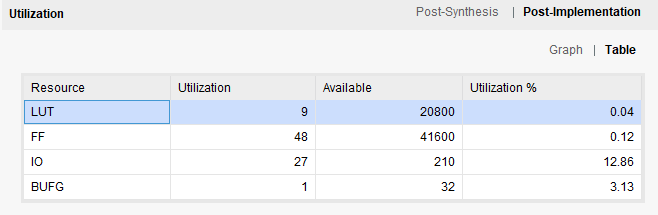
\includegraphics[width=0.7\textwidth]{image/2024-06-17-17-00-36.png}
    \caption{资源使用}
    \label{image_30Hz_utilization}
\end{figure}
该部分资源使用如图\ref{image_30Hz_utilization}所示, 使用资源极少, 但实现了极高分辨率的任意频率生成。
\subsection*{提高任务}
偶数分频器设计源文件如下:
\begin{lstlisting}[language=Verilog, caption={通用偶数分频器源文件}]
module clk_div_even(
    input clk,
    input rst,
    input [7:0] div_N,
    output clk_out
    );
    /* 操作cnt */
    reg [7:0] cnt;
    always @(posedge clk, posedge rst) begin
        if (rst) begin
            cnt <= 8'b0;
        end
        else if (cnt < {div_N[7:1], 1'b0} - 1'b1) begin
            cnt <= cnt + 1'b1;
        end
        else begin
            cnt <= 8'b0;
        end
    end
    assign clk_out = (cnt < {1'b0, div_N[7:1]}) ? 1'b1 : 1'b0;
endmodule    
\end{lstlisting}
偶数分频器设计的过程中, 首先要保证时序逻辑的复位功能有效, 提供对复位的支持, 实现异步的高电平复位。计数器在计数的过程中, 总计计数分频系数次的输入周期,
对应的计数器值为0~N-1, 之后利用assign设计计数值映射为输出时钟0和1的逻辑电路即可。
\begin{lstlisting}[language=Verilog, caption={偶数分频器仿真激励}]
initial begin
    div_coe = 8'd12;
    clk = 0;
    rst = 0;
    #100;
    rst = 1;
    #10;
    rst = 0;
end
\end{lstlisting}
\subsection*{拓展任务}
奇数分频器采用两个计数器和或运算实现, 具体原理可见设计内容分析。
实现的奇数分频其源文件如下:
\begin{lstlisting}[language=Verilog, caption={通用奇数分频器设计源文件}]
module clk_div_odd(
    input clk,
    input rst,
    input [7:0] div_N,
    output clk_out
    );

    /* 保证输入分频系数为奇数 */
    wire [7:0] div_N_in;
    assign div_N_in = div_N | 8'b0000_0001;

    /* 第一个计数器, 采样上升沿 */
    reg [7:0] cnt1;
    always @(posedge clk, posedge rst) begin
        if (rst) begin                          /* 高电平异步复位 */
            cnt1 <= 8'b0;
        end
        else if(cnt1 < div_N_in-1'b1) begin    /* 已采样N次上升沿 */
            cnt1 <= cnt1 + 1'b1;
        end
        else begin                              /* 采样自增 */
            cnt1 <= 8'b0;
        end
    end
    assign clk1 = (cnt1 < {1'b0, div_N_in[7:1]}) ? 1'b1 : 1'b0; /* 高电平比低电平多1个周期 */
    
    /* 第二个计数器, 采样下降沿 */
    reg [7:0] cnt2;
    always @(negedge clk, posedge rst) begin
        if (rst) begin                          /* 高电平异步复位 */
            cnt2 <= 8'b0;
        end
        else if(cnt1 < div_N_in-1'b1) begin    /* 已采样N次下降沿 */
            cnt2 <= cnt2 + 1'b1;
        end
        else begin                              /* 采样自增 */
            cnt2 <= 8'b0;
        end
    end
    assign clk2 = (cnt2 < {1'b0, div_N_in[7:1]}) ? 1'b1 : 1'b0; /* 高电平比低电平多一个周期 */
    assign clk_out = clk1 | clk2;               /* 通过或运算输出.5周期结果 */
endmodule
\end{lstlisting}
二进制转BCD码源文件如下:
\begin{lstlisting}[language=Verilog, caption={二进制转BCD码}]
module bin2bcd_8bit(
    input [7:0] bin, 
    output [3:0] bcd_12bit  /* 高中低BCD结果 */
    );

    integer i;
    reg [19:0] bcd_temp;
    always @(*) begin
        // 初始化, 直接移位三次
        bcd_temp = {9'b0, bin, 3'b0};
        // 逐位移位法
        for (i = 0; i < 5; i = i + 1'b1) begin
            // 如果BCD的每一部分 > 4,加3
            if (bcd_temp[11:8] > 4)
                bcd_temp[11:8] = bcd_temp[11:8] + 3;
            if (bcd_temp[15:12] > 4)
                bcd_temp[15:12] = bcd_temp[15:12] + 3;
            if (bcd_temp[19:16] > 4)
                bcd_temp[19:16] = bcd_temp[19:16] + 3;
            // 左移1位
            bcd_temp = {bcd_temp[18:0], 1'b0};
        end
    end
    assign bcd_12bit = bcd_temp[19-:12];
endmodule
\end{lstlisting}
数码管显示源文件如下:
\begin{lstlisting}[language=Verilog, caption={数码管显示源文件}]
module scan_led_hex_disp_4(
    input clk, rst,
    input [3:0] hex0, hex1, hex2, hex3, /* 显存 */
    input [3:0] dp,
    output reg [3:0] an,
    output reg [7:0] sseg
    );

    localparam N = 16 + 2;              /* 100MHz时钟分频, 100Mhz/ 2^16 */         
    reg [N-1:0] regN;

    always @(posedge clk, posedge rst) begin
        if (rst)
            regN <= 0;
        else 
            regN <= regN + 1;
    end

    always @(*) begin
        case (regN[N-1:N-2])
            2'b00: begin
                an <= 4'b0001;
                sseg[6:0] <= dt_translate(hex0);
                sseg[7] <= dp[3];
            end
            2'b01: begin
                an <= 4'b0010;
                sseg[6:0] <= dt_translate(hex1);
                sseg[7] <= dp[2];
            end
            2'b10: begin
                an <= 4'b0100;
                sseg[6:0] <= dt_translate(hex2);
                sseg[7] <= dp[1];
            end
            2'b11: begin
                an <= 4'b1000;
                sseg[6:0] <= dt_translate(hex3);
                sseg[7] <= dp[0];
            end 
        endcase
    end

    function [6:0] dt_translate;
        input [3:0] data;
        begin
            case(data)
                4'd0: dt_translate = 7'b1111110;     //number 0 -> 0x7e
                4'd1: dt_translate = 7'b0110000;     //number 1 -> 0x30
                4'd2: dt_translate = 7'b1101101;     //number 2 -> 0x6d
                4'd3: dt_translate = 7'b1111001;     //number 3 -> 0x79
                4'd4: dt_translate = 7'b0110011;     //number 4 -> 0x33
                4'd5: dt_translate = 7'b1011011;     //number 5 -> 0x5b
                4'd6: dt_translate = 7'b1011111;     //number 6 -> 0x5f
                4'd7: dt_translate = 7'b1110000;     //number 7 -> 0x70
                4'd8: dt_translate = 7'b1111111;     //number 8 -> 0x7f
                4'd9: dt_translate = 7'b1111011;     //number 9 -> 0x7b
            endcase
        end
    endfunction
endmodule
\end{lstlisting}
top源文件如下:
\begin{lstlisting}[language=Verilog, caption={top源文件}]
module clk_div_top(
    input clk,                  /* 100MHz */
    input rst,                  /* 低电平异步复位 */
    input [7:0] div_coe,        /* 输入的四位整数加四位小数的二进制实数 */
    output [7:0] sseg1, sseg2,  /* 八段数码管 */
    output [3:0] an1, an2,      /* 片选信号 */
    output led_out              /* 闪烁的LED灯 */
    );

    /* 分频产生30Hz */
    wire clk_30Hz;
    clk_div_32bit  clk_div_32bit_inst (
        .clk(clk),
        .rstn(!rst),
        .step_freq(32'd1288),
        .clk_out(clk_30Hz)
    );

    wire clk_out_even;
    clk_div_even  clk_div_even_inst (
        .clk(clk_30Hz),
        .rst(rst),
        .div_N(div_coe),
        .clk_out(clk_out_even)
    );

    wire clk_out_odd;
    clk_div_odd  clk_div_odd_inst (
        .clk(clk_30Hz),
        .rst(rst),
        .div_N(div_coe),
        .clk_out(clk_out_odd)
    );

    /* 检测输入状态, 当分频系数输入为0或1, 认为不分频, 显示30Hz的分频系数 */
    assign div_none = div_coe < 8'd2 ? 1'b1 : 1'b0;

    /* 根据输入系数切换输出 */
    assign led_out = div_none ? clk_30Hz :
                        (div_coe[0]) ? clk_out_odd : clk_out_even;

    wire [11:0] bcd_12bit;
    bin2bcd_8bit  bin2bcd_8bit_inst (
        .bin(div_coe),
        .bcd_12bit(bcd_12bit)
    );

    /* 修改显示内容 */
    reg [3:0] disp_buffer[0:7];
    always @(*) begin
        if (div_none) begin
            disp_buffer[0] <= 4'd3;
            disp_buffer[1] <= 4'd3;
            disp_buffer[2] <= 4'd3;
            disp_buffer[3] <= 4'd4;
            disp_buffer[4] <= 4'd6;
            disp_buffer[5] <= 4'd0;
            disp_buffer[6] <= 4'd1;
            disp_buffer[7] <= 4'd9;
        end
        else begin
            disp_buffer[0] <= 4'd0;
            disp_buffer[1] <= 4'd0;
            disp_buffer[2] <= 4'd0;
            disp_buffer[3] <= 4'd0;
            disp_buffer[4] <= 4'd0;
            disp_buffer[5] <= bcd_12bit[11:8];
            disp_buffer[6] <= bcd_12bit[7:4];
            disp_buffer[7] <= bcd_12bit[3:0];            
        end
    end

    /* 修改小数点 */
    reg [3:0] dot_buffer;
    always @(*) begin
        if (div_none) begin
            dot_buffer <= 4'b0010;
        end
        else begin
            dot_buffer <= 4'b0000;
        end
    end

    /* 第一个四位数码管 */
    scan_led_hex_disp_4  scan_led_hex_disp_4_inst_0 (
        .clk(clk), .rst(rst),
        .hex0(disp_buffer[0]), .hex1(disp_buffer[1]), .hex2(disp_buffer[2]), .hex3(disp_buffer[3]), .dp(4'b0000),
        .an(an1), .sseg(sseg1)
    );
    /* 第二个四位数码管 */
    scan_led_hex_disp_4  scan_led_hex_disp_4_inst_1 (
        .clk(clk), .rst(rst),
        .hex0(disp_buffer[4]), .hex1(disp_buffer[5]), .hex2(disp_buffer[6]), .hex3(disp_buffer[7]), .dp(dot_buffer),
        .an(an2), .sseg(sseg2)
    );
endmodule
\end{lstlisting}
奇数分频器设计过程中的仿真激励如下:
\begin{lstlisting}[language=Verilog, caption={奇数分频器仿真激励}]
initial begin
    div_coe = 8'd7;
    clk = 0;
    rst = 0;
    #100;
    rst = 1;
    #10;
    rst = 0;
end
\end{lstlisting}
整个系统的仿真文件如下:
\begin{lstlisting}[language=Verilog, caption={Top系统仿真文件如下}]
module clk_div_top_tb_1;
    reg  clk;
    reg  rst;
    reg [7:0] div_coe;
    wire [7:0] sseg1, sseg2;
    wire [3:0] an1, an2;
    wire  led_out;

    initial begin
        clk = 0;
        rst = 0;
        #10;
        rst = 1;
        #10;
        rst = 0;

        div_coe = 8'd0;
        #300_000_000;
        div_coe = 8'd4;
        #300_000_000;
        div_coe = 8'd5;
        #300_000_000;
        $finish;
    end

    clk_div_top  clk_div_top_inst (
        .clk(clk),
        .rst(rst),
        .div_coe(div_coe),
        .sseg1(sseg1),
        .sseg2(sseg2),
        .an1(an1),
        .an2(an2),
        .led_out(led_out)
    );

    always #5 clk = ! clk ;
endmodule
\end{lstlisting}
% 第三部分
\section*{\fourhao 三、仿真结果}
\xiaosihao
\setstretch{1.5}
% 对仿真图像要有解释,要对所有的可能性进行标注及解释
% 按照基础任务、提高任务和拓展任务分别给出仿真结果
\subsection*{基础任务}
\begin{figure}[H]
    \centering
    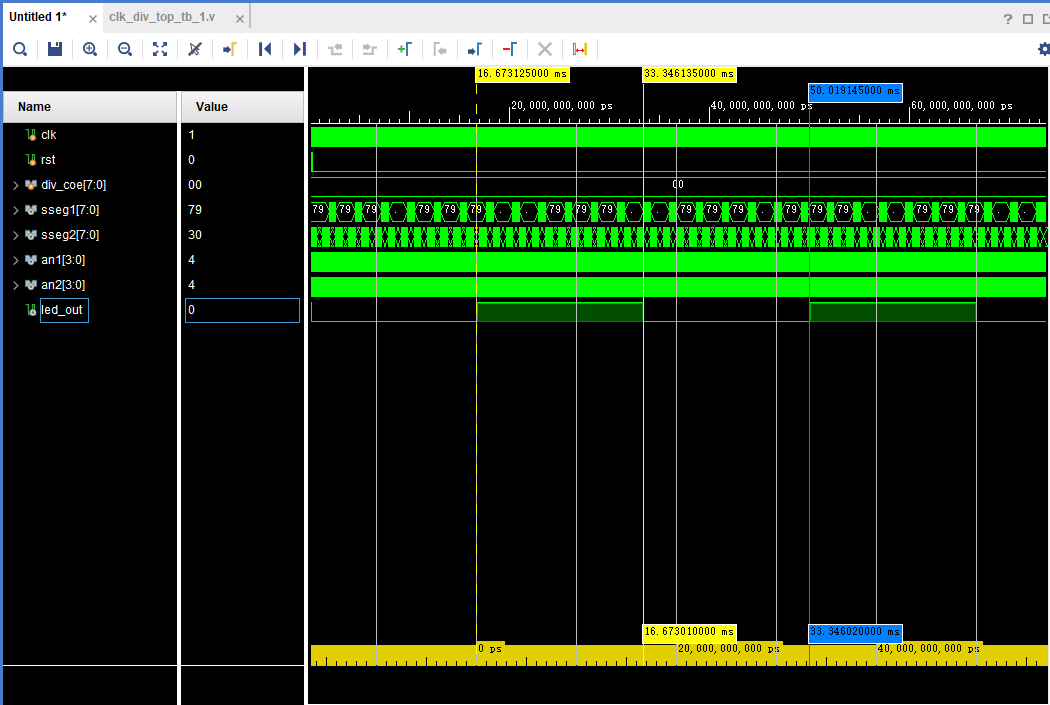
\includegraphics[width=0.7\textwidth]{image/2024-06-17-16-01-30.png}
    \caption{30Hz输出仿真结果}
    \label{image_30Hz_sim}
\end{figure}
输出30Hz的仿真结果见图\ref{image_30Hz_sim}, 首先可以通过Marker看到, 在一个输出时钟周期内, 信号的时钟周期为50\%占空比, 周期为33.346ms, 计算得到其频率为29.9866Hz, 与理论计算结果一致。
\begin{equation}
    f = \frac{1}{33.346*10^{-3}} = 29.9886Hz
\end{equation}
\subsection*{提高任务}
\begin{figure}[H]
    \centering
    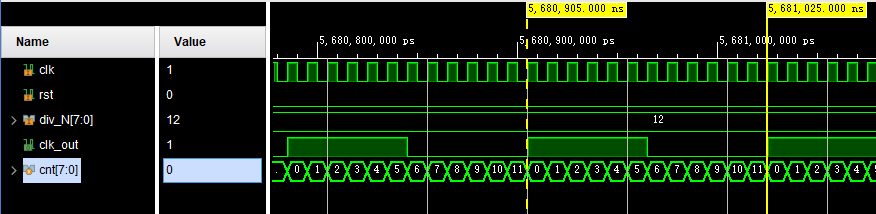
\includegraphics[width=0.7\textwidth]{image/2024-06-18-14-20-51.png}
    \caption{偶数分频仿真结果}
    \label{image_even_sim}
\end{figure}
对偶数分频器的仿真如图\ref{image_even_sim}所示, tb文件中设定了输入的分频系数为12, 仿真结果可以清晰地看到, 分频产生的输出时钟的周期为12个输入时钟, 并且其占空比为\%50。
\subsection*{拓展任务}
\begin{figure}[H]
    \centering
    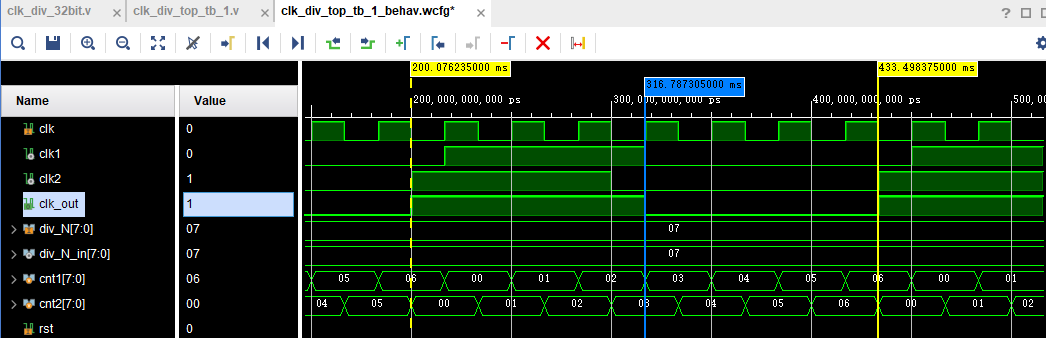
\includegraphics[width=0.7\textwidth]{image/2024-06-18-16-01-10.png}
    \caption{奇数分频器仿真结果}
    \label{image_odd_sim}
\end{figure}
对奇数分频器的仿真如图\ref{image_odd_sim}所示, tb文件中设定了输入的分频系数为7, 对输入时钟进行7分频, 结果应该是输出时钟的高低电平各包含3.5周期, 通过仿真时序图可以清晰地看到, 输出波形clk\_out高低电平各为3.5周期, 达到了50\%占空比的分频输出要求。
\begin{figure}[htbp]
    \centering
    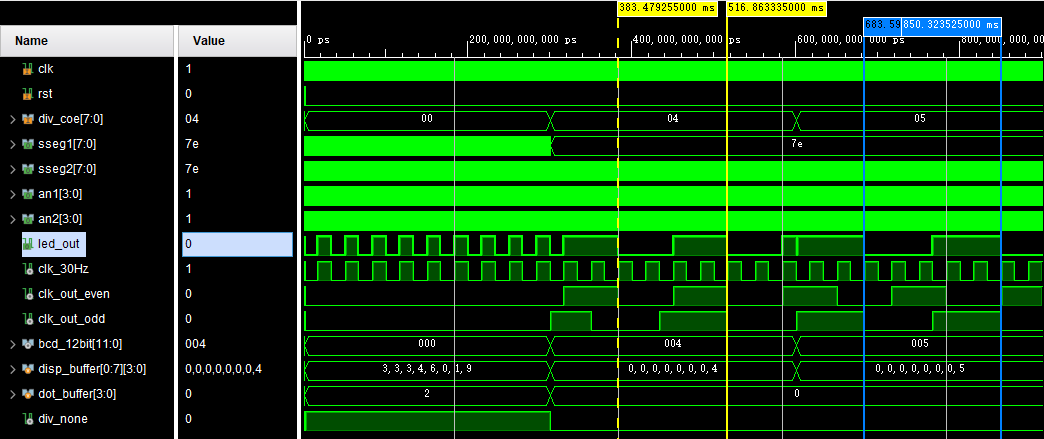
\includegraphics[width=0.7\textwidth]{image/2024-06-18-17-07-24.png}
    \caption{Top系统仿真结果}
    \label{image_top_sim}
\end{figure}
top系统的仿真结果如图\ref{image_top_sim}所示, 前300ms为输出30Hz分频信号, 同时显示其系数, 之后一个300ms内将分频系数设置为4, 系统将输出信号切换为偶分频器输出结果, 最后300ms内, 将分频系数设置为5, 数码管将显示005, 同时自动输出奇数分频产生5分频信号, 频率在6Hz左右。
% 第四部分
\section*{\fourhao 四、硬件验证结果}
\xiaosihao
\setstretch{1.5}
% 记录加编程器与拨码开关和发光二极管、数码管等的连接情况。记录开发板硬件验证结果,并分析其结果的正确性。
% 按照基础任务、提高任务和拓展任务分别分析
\subsection*{基础任务}
\begin{figure}[H]
    \centering
    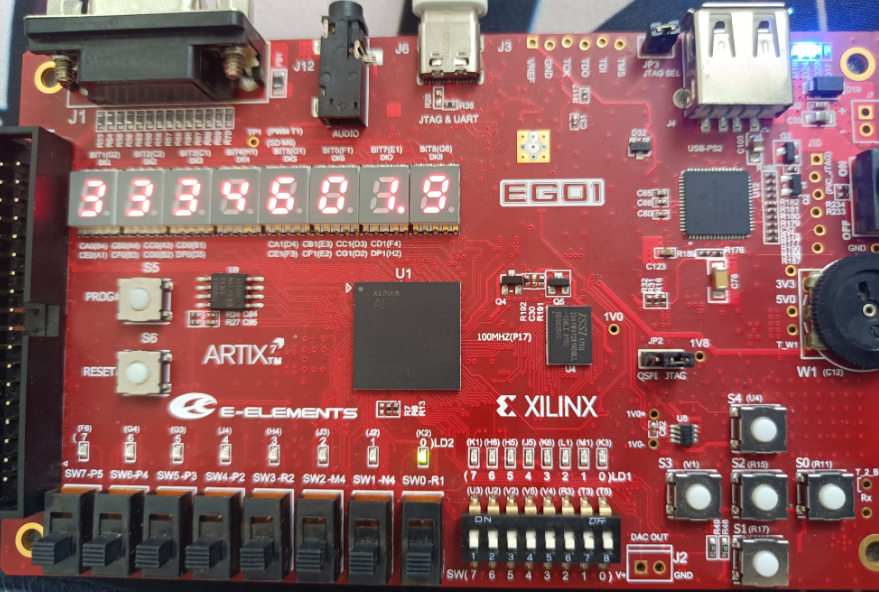
\includegraphics[width=0.7\textwidth]{image/2024-06-18-09-38-37.png}
    \caption{30Hz输出时钟的硬件验证}
    \label{image_30Hz_verify}
\end{figure}
硬件验证结果如图\ref{image_30Hz_verify}所示, 数码管能够正确显示对应的分频系数, 肉眼能够观察到对应的LD2\_2频闪。
\subsection*{提高任务}
\begin{figure}[H]
    \centering
    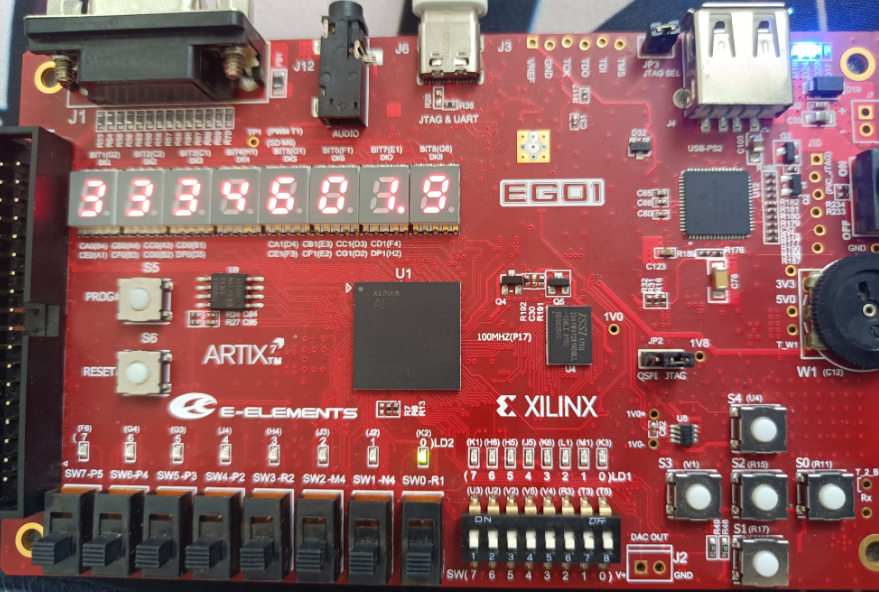
\includegraphics[width=0.7\textwidth]{image/2024-06-18-09-38-37.png}
    \caption{偶分频的硬件验证}
    \label{image_even_verify}
\end{figure}
硬件验证结果如图\ref{image_even_verify}所示, 通过拨码开关设置分频系数为28进行偶分频, 数码管显示正确, 可以明显通过肉眼观察到LED的亮灭变化, 相比于30Hz已经进一步分频为
$$f_o = \frac{29.9886}{28}(Hz) = 1.0710 (Hz)$$
\subsection*{拓展任务}
\begin{figure}[htbp]
    \centering
    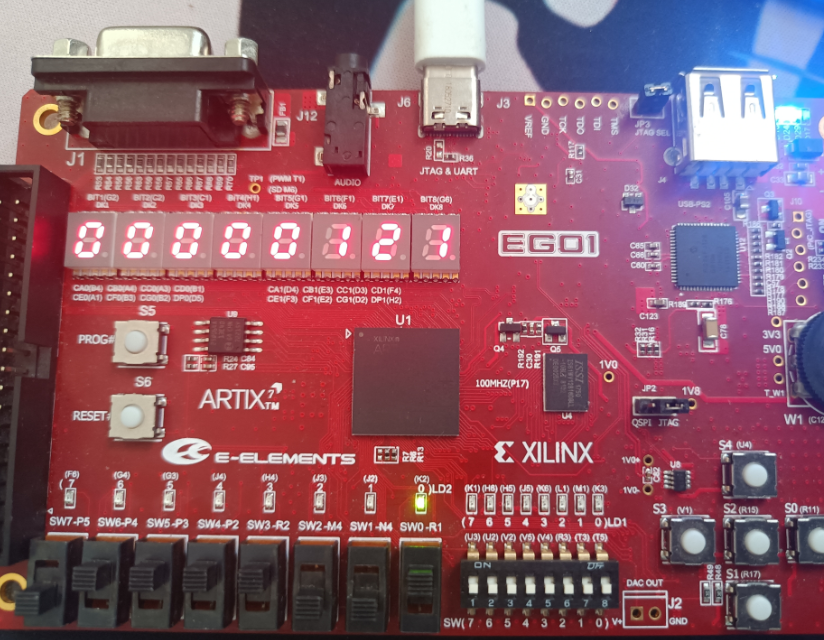
\includegraphics[width=0.7\textwidth]{image/2024-06-18-18-43-30.png}
    \caption{奇分频硬件验证}
    \label{image_odd_verify}
\end{figure}
硬件验证结果如图\ref{image_even_verify}所示, 通过拨码开关设置分频系数为121进行奇分频, 数码管显示正确, 可以明显观察到LED的缓慢的进行亮灭变化, 相比于30Hz已经进一步分频为
$$f_o = \frac{29.9886}{121}(Hz) = 0.24784 (Hz)$$
% 第五部分
\section*{\fourhao 五、问题解决}
\xiaosihao
\setstretch{1.5}
% 设计过程中遇到的问题及解决的方法。
\subsection*{最后系统设计中, 偶分频不输出}
\begin{figure}[H]
    \centering
    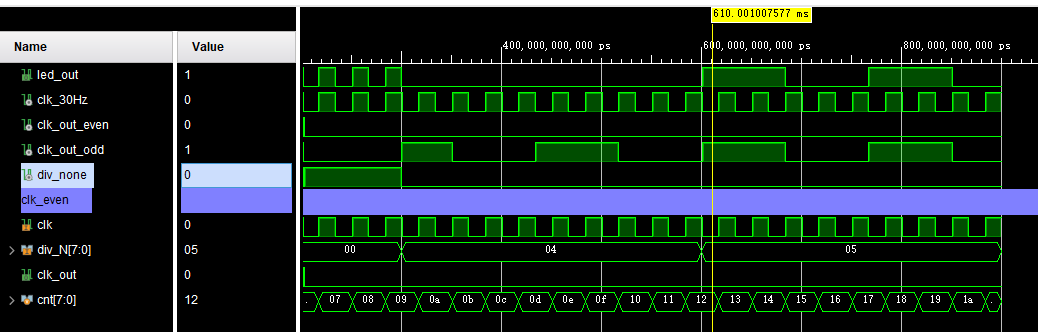
\includegraphics[width=0.7\textwidth]{image/2024-06-18-16-29-13.png}
    \caption{问题仿真}
    \label{image_QA_1}
\end{figure}
通过系统仿真, 观察通用偶分频器模块内部计数器变化解决问题, 仿真结果如图\ref{image_QA_1}所示, 仿真文件中给了300ms时间用于偶分频输出, 通过观察内部计数器的变化可以得知, 源文件设计为到达目标值时复位, 但是cnt没有进行使能管理, 导致cnt在进行有效分频前就进行了采样计数, 导致其计数值大于了设定的溢出值, 计数器来不及溢出清零。
将分频器中计数器的清零判断由相等改为小于则增判断。
% 第六部分
\section*{\fourhao 六、心得体会}
\xiaosihao
\setstretch{1.5}
时序逻辑设计是复杂系统设计过程中所必需的, 通过分频器的设计流程, 同时掌握了DDS数字电路部分的技术原理和计数器的应用, 
在理解和掌握这些原理的基础, 将其用Verilog语言描述并实现自己的想法, 实现任意分频模块, 并完成偶分频和奇分频的通用模
块这些时序电路中基础, 对之后更加复杂的电路设计奠定了基础。并通过适当扩展, 将偶分频和奇分频模块结合后, 实现任意整数
分频, DDS的相位累加器则可以实现小数分频。\\

随着设计越来越复杂, 所使用的模块也越来越多, 体现出了层次化设计的强烈需求, 可以适当通过IP封装, 提高模块的复用效率。
\end{document}